%
% nonlinear.tex -- XXX
%
% (c) 2019 Prof Dr Andreas Mueller, Hochschule Rapperswil 
%
\chapter{Nonlinear partial differential equations
\label{chapter:nichtlinear}}
\lhead{Nonlinear partial differential equations}
\rhead{}
Die Grundgleichungen der Elektrodynamik und der Elastizitätstheorie
sind linear. Die in den vorangegangenen Kapiteln dargestellten
Lösungensmethoden sind auf derartige Differentialgleichungen
zugeschnitten. Einige bedeutenden Probleme der Naturwissenschaften
führen dagegen auf nichtlineare Gleichungen, für die die
Methoden ungeeignet sind. In diesem Kapitel werden einige
solche Gleichungen vorgeführt und die dabei auftretenden
Schwierigkeiten illustriert.

%
% examples.tex
%
% (c) 2019 Prof Dr Andreas Mueller
%
\chapter{Introductory examples of partial differential equations
\label{chapter:examples}}
\lhead{Introductory examples}
In this chapter we present a few partial differential equations
of prime practical importance which will also serve us as case
studies to illustrate general theorems and solution techniques.
The examples illustrate
\begin{enumerate}
\item
the manifold applications of the theory of partial differential equations,
\item
three completely different cases that lead to incompatible solution
algorithms and
\item
the importance of boundary and initial conditions.
\end{enumerate}

%
% waveequation.tex -- the wave equation
%
% (c) 2019 Prof Dr Andreas Mueller
%
\rhead{Wave equation}
\section{Wave equation\label{beispiele:wellengleichung}}
\index{wave equation}
In the simplest form, this equation describes the motion
of a string of a guitar or a piano, or the air column of a 
wind instrument.
It can be generalized to vibration of a membrane or the fluid inside
an arbitrary threedimensional volume.
Electromagnetic waves can be modelled with this equation just as
well as the waves on the surface of a lake.

\subsection{The differential equation of a vibrating string}
\index{string}
Let a thin string with linear mass density $\mu$ be mounted between
the points $x=0$ and $x=l$ (figure~\ref{saite}).
The force $F$ at the end points of the string maintains its tension.
We ask for a partial differential that describes the motion of a
string after we bring it into a certain shape and let it go at time $t=0$.

The state of the string at any time can be described by a function
$u(x,t)$, which measures the deflection of the string from the straight
line between the two end points.
We need to find a differential equation for the function $u$.

From this problem description we can already derive some information
about the solution.
We note that the end points of the string are fixed, so
\[
u(0,t)=u(l,t)=0\quad\forall t\ge 0.
\]
We call this a boundary condition.
At time $t=0$ the string is supposed to have a given shape.
This is the situation of the guitar player who plucks a string and then
lets it go.
Mathematically we can formulate this as the initial condition
\[
u(x,0) = f(x)\qquad 0 < x < l.
\]
A piano however works differently, at $t=0$ it imparts a certain velocity
profile on the string, or in mathematical form
\[
\frac{\partial}{\partial t}u(0,x) = g(x),\qquad 0<x<l.
\]

\begin{figure}
\begin{center}
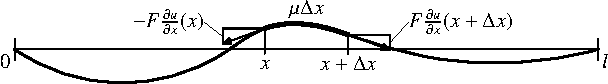
\includegraphics[width=\hsize]{../common/images/saite-1}
\end{center}
\caption{Derivation of the differential equation of a vibrating string
\label{saite}}
\end{figure}
To derive the equation of motion of a vibrating string, we consider
a small section of the string between coordinates $x$ and $x+\Delta x$
(figure \ref{saite}).
Newton's law says that the acceleration of this piece of string 
is proportional to forces acting on it, with the mass as proportionality
factor.
The mass of this piece of the string is $m=\mu\Delta x$.
At each end of the segment, a force of absolute value $F$ pulls the piece
outward, but these forces don't necessarily have the same direction,
resulting in a vertical force component.
This component turns out to be
\[
F\frac{\partial u}{\partial x}(x+\Delta x)-F\frac{\partial u}{\partial x}(x).
\]
Since the acceleration of the string segment is
$\displaystyle\frac{\partial^2u}{\partial t^2}$
we obtain the equation of motion
\begin{align*}
\mu\Delta x\frac{\partial^2u}{\partial t^2}(x)&=
F\frac{\partial u}{\partial x}(x+\Delta x)-F\frac{\partial u}{\partial x}(x)\\
\Rightarrow\qquad
\frac{\mu}{F}\frac{\partial^2u}{\partial t^2}(x)&=
\frac1{\Delta x}\left(\frac{\partial u}{\partial x}(x+\Delta x)-\frac{\partial u}{\partial x}(x)\right)
\end{align*}
By going to the limit 
$\Delta x\to 0$ we obtain the partial differential equation
\begin{equation}
\frac{\partial^2u}{\partial t^2}=\frac{F}{\mu}\frac{\partial^2u}{\partial x^2}.
\label{examples:wave-equation}
\end{equation}
This is the wave equation.
The coefficient
$\frac{F}{\mu}$
in \eqref{examples:wave-equation}
has the dimension of a velocity squared, it is the velocity by which waves
propagate along the string.

\subsection{The differential equation of an organ pipe}
\index{organ pipe}
The analysis of the vibrating string carries over almost unchanged
to a pipe organ (or any other wind instrument).
The deflection of the string is replaced by a deviation of the pressure.
We then obtain the wave equation
\[
\frac{\partial^2p}{\partial t^2}=
a^2\frac{\partial^2p}{\partial x^2}
\]
Again, $a$ is the velocity by which pressure changes propagate in
the medium, i.~e.~the speed of sound.

The boundary conditions, however, turn out to be more complicated and more
interesting.
If the end of the pipe is closed, then the air cannot move at this end.
Because movement of the air in the pipe is always associated with pressure
differences, we conclude that there cannot be a pressure gradient at the
end of the pipe in this case.
This leads to the so called {\em Neumann boundary condition}
\index{Neumann boundary conditions}
\[
\frac{\partial}{\partial x}p(x_0,t) = 0\qquad \text{for $t>0.$}
\]

On the other hand, if the pipe is open, then there is nothing that keeps
the air in the pipe, air can move freely, and the pressure is always equal
to that the surrounding air.
This leads to the so called {\em Dirichlet boundary condition}
\index{Dirichlet boundary conditions}
\[
u(x_0,t)=0\qquad \text{for $t>0.$}
\]

\subsection{Wave equation in two and three dimensions}
In analogy with the differential equation of a string we can derive the
equation of motion of a membrane fixed around its perimeter.
\index{membrane}
Let $G$ be a two-dimensional domain\footnote{The precise definition of
the term {\em domain} will be given later.}
in $\mathbb R^2$ describing the shape
of the membrane, and let $\gamma=\partial G\subset G$ be
the boundary curve of the domain.
Then the deviation of the membrane from zero position is a function
\[
 u \colon G\times \mathbb R_{t \ge 0}\to\mathbb R\colon (x,y,t)\mapsto  u (x,y,t)
\]
The membrane is fixed at the boundary, so $u$ has to satisfy the
boundary conditions
\[
 u (x,y,t)=0\qquad \forall (x,y)\in\partial G,\quad t\ge 0.
\]
The function satisfies the partial differential equation
\[
\frac{\partial^2 u }{\partial t^2}
=
c^2\left(\frac{\partial^2 u }{\partial x^2}
+
\frac{\partial^2 u }{\partial y^2}\right)
\qquad\text{in $G$.}
\]
The solution is only determined if we know the initial shape of the
membrane and its velocity. 
This leads to the initial conditions
\begin{equation}
\left.
\begin{aligned}
 u (x,y,0)&=f(x,y)
\frac{\partial}{\partial t} u(x,y,0)=g(x,y)
\end{aligned}
\right\}\qquad
\forall (x,y)\in G.
\end{equation}

In three dimensions, the wave equation becomes
\[
\frac{\partial^2 u }{\partial t^2}
=c^2\left(\frac{\partial^2 u }{\partial x^2}
+\frac{\partial^2 u }{\partial y^2}
+\frac{\partial^2 u }{\partial z^2}
\right).
\]
The additional data required also becomes a bit more involved.
First we have to define a domain 
$G\subset \mathbb R^3$ in threedimensional space.
The boundary of this volume must be a sufficiently smooth surface.
The solution then has to satisfy the boundary conditions
$u(x,y,z,t) = 0$ for points
$(x,y,z)\in \partial G$ on the boundary surface of $G$.

\subsection{The Laplace operator\label{beispiele:laplaceoperator}}
\index{Laplace operator}
\index{laplacian}
In all the problems discussed so far, the Laplace operator,
also called laplacian,
\[
\Delta
=
\begin{cases}
\displaystyle
\frac{\partial^2}{\partial x^2}
+\frac{\partial^2}{\partial y^2}&\qquad\text{two dimensions}\\
\\
\displaystyle
\frac{\partial^2}{\partial x^2}
+\frac{\partial^2}{\partial y^2}
+\frac{\partial^2}{\partial z^2}&\qquad\text{three dimensions}
\end{cases}
\]
appeared.
In fact, up to a constant factor, it turns out that this is the only
linear operator involving only second derivatives that is invariant
with respect to arbitrary rotations of the coordinate system.
This means that for a problem that is rotationally symmetrc, this is
the only operator that can have a physical meaning independent
of the choice of coordinate system.


%
% poissonproblem.tex
%
% (c) 2019 Prof Dr Andreas Mueller
%
\section{Poisson problem}
\rhead{Poisson problem}
\label{poisson-problem}
This section describes two examples of elliptic partial differential
equations, to be expanded on in chapter~\ref{chapter-elliptisch}.

\subsection{Minimal surfaces\label{beispiele:minimal surfaces}}
What shape will a soap film take when it is lifted to height
$f(x,y)$ at the boundary $(x,y)\in\gamma$ of 
a two dimensional domain $G\subset \mathbb R^2$?
If we describe the height of the soap film using a function
$u(x,y)$, we expect to find a partial differential equation for $u$
with boundary condition $f$.
\index{minimal surface}

In the derivation of the equation of motion for the vibrating string
we learned that the force accelerating the string depended on the
curvature of the string.
For the soap film, the restoring force is provided by the surface
tension which is equally strong in each direction of the film.
The soap film has two directions in which it can curve, roughly
given by the second partial derivatives $\partial^2 u/\partial x^2$ and
$\partial^2 u/\partial y^2$.
We therefore expect that force accelerating the film proportional
to the sum of these second derivatives with respect to $x$ and $y$.
Since the film is supposed not to move, we expect the differential
equation:
\[
\frac{\partial^2 u }{\partial x^2}+\frac{\partial^2 u }{\partial y^2}
=\Delta u =0.
\]

This simplified derivation is only valid for small deviations.
More generally, the so called mean curvature of the surface needs
to vanish for a minimal surface.
\index{mean curvature}

\subsection{Electric potential}
\index{electric potential}
In electrodynamics it is shown that a static electric field is a 
gradient field, i.~e.~there is a potential $\varphi$ such that the
electric field
\[
\vec E=\operatorname{grad}\varphi
\]
is its gradient.
It is also shown that the sources of the field are the electric charges.
Without charges, there are no sources to the field.
The mathematical expression of these facts is that 
the electric field satisfies the same partial differential equation
\[
\operatorname{div}\vec E=\operatorname{div}\operatorname{grad}\varphi
=\Delta \varphi=0
\]
as a minimal surface.
This problem seems to have mathematical significance independent of the
particular application.


%
% heatequation.tex -- heat equation
%
% (c) 2008 Prof Dr Andreas Mueller
%
\rhead{Heat equation}
\section{Heat equation}
The heat equation is a prototype for a so called parabolic differential
equation.
Such equations are also used to describe diffusion processes.
The Schrödinger equation, the basis of quantum mechanics, is also of this type.

We derive the heat equation for the one dimensional case.
We examine a rod of length $l$ between $x$-coordinates $0$ and $l$
and strive to compute the temperature distribution $T(x,t)$ for 
$0<x<l$ and for all times $t>0$.
We need the initial temperature distribution, which we call
$T(x,0) = f(x)$.
We expect to solve this problem using a partial differential equation.

The heat that flows in a time interval $\Delta t$ through the rod at
coordinate $x$ is proportional to the temperature gradient at that point.
The amount of heat flowing into the section  of the rod between
$x$ and $x+\Delta x$ is therefore proprtional to
\[
\frac{\partial T}{\partial x}(x+\Delta x)-\frac{\partial T}{\partial x}(x).
\]
This additional heat lets the temperature if the segment rise, depending
on the heat capacity of the material.
The volume of the segment is $\Delta x$, the temperature change is smaller
when the volume is larger.
It becomes
\[
\Delta T
=
\kappa
\frac{1}{\Delta x}
\biggl(
\frac{\partial T}{\partial x}(x+\Delta x)-\frac{\partial T}{\partial x}(x).
\biggr) \Delta t.
\]
Dividing by $\Delta t$ and going to the limits $\Delta t\to 0$
and $\Delta x\to 0$ leads to
\[
\lim_{\Delta t\to 0}\frac{\Delta T}{\Delta t}
=
\frac{\partial T}{\partial t}
=
\kappa
\lim_{\Delta x\to 0}\frac1{\Delta x}\left(\frac{\partial T}{\partial x}(x+\Delta x)-\frac{\partial T}{\partial x}(x)\right)
=\kappa\frac{\partial^2T}{\partial x^2}.
\]

Again we have to specify suitable initial and boundary conditions.
As initial condition we already have found
\[
T(x,0)=f(x)\qquad \forall x\in[0,l].
\]
As a boundary condition at the end of the rod we could prescribe the
temperature.
In physics terms this means that both ends of the rod are in contact
with a heat reservoir at constant temperature.
If we prescribe the derivatives of $T$ with respect to $x$ at $x=0$ and
$x=l$, we fix the flow of heat into the rod.
In particular, requiring
\[
\frac{\partial T}{\partial x} = 0
\]
means that no heat flows through the ends of the rod, the rod is
thermally isolated from its environment.


%
% supersonic.tex -- the equation for a supersonic flow
%
% (c) 2008 Prof Dr Andreas Mueller
%
\rhead{Supersonic flow}
\section{Supersonic flow}
In the year 1928, Jakob Ackeret habilitated at ETH Zürich with a 
\index{Ackeret, Jakob}
\index{supersonic flow}
paper with the title
``Über Luft-Kräfte bei sehr grossen
Geschwindigkeiten insbesondere bei ebenen Strömungen''.
He showed how to compute the aerodynamic forces on an object
in a supersonic flow using a linear approximation.
The velocity field of the gas that enters the region of interest with
velocity $v_1$ in $x$-direction turns out to be the gradient of
a function $\varphi(x,y,z)$ that satisfies the equation
\[
(1-\textit{Ma}_1)\frac{\partial^2\varphi}{\partial x^2}
+
\frac{\partial^2\varphi}{\partial y^2}
+
\frac{\partial^2\varphi}{\partial z^2}=0.
\]
The expression
$\textit{Ma}_1=\frac{v_1}{c_1}$ is called the Mach number of the flow,
$c_1$ is the speed of sound.
The Mach number expresses the flow velocity in units of the speed of sound.

For small velocities, we have $(1-\textit{Ma}_1)>0$, and the equation
becomes similar to the Poisson problem.
This is called potential flow.

For supersonic flow, however, the first term
$(1-\textit{Ma}_1) < 0$
changes sign, and the equation behaves like a wave equation.
In fact, the flow shows shock waves propagating away from the object
and thus carrying away its energy
(figure~\ref{ueberschall2d}).
By carefully analyzing this solution, Ackeret was able to compute
aerodynamic drag due to these shock waves.
\index{areodynamic drag}
\index{shock waves}


%
% beamequation.tex -- beam equation
%
% (c) 2019 Prof Dr Andreas Mueller
%
\rhead{Beam equation}
\section{Beam equation}
In the derivation of the differential equation of a string we
have used that fact that the string does not resist to being
bent.
Even large curvature of the string does not result in force trying
to straighten it out again.
A beam behaves completely differently.
Bending the beam creates internal stresses in the beam that
try to bring the beam back to its original shape.
We don't try to explain these forces, but it is natural to expect that
they will be proportional to the curvature and thus to the second
derivatives of the beam.
In addition, the are proportional to some material constants
(the elastic modulus $E$)
and to a property derived from the cross section of the beam,
namely the second moment $I$%
\footnote{The definition of $I$ is not relevant for the present
discussion.}.

A segment of length $\Delta x$ of a beam with linear mass density $m$
therefore experiences the following force components:
\begin{enumerate}
\item
Restoring forces caused by the stresses in the beam:
$-EI\frac{\partial^4}{\partial^4 x}w(t,x)\Delta x$
\item
Damping
$-b\frac{\partial}{\partial t}w(t,x)\Delta x$
\item
Exterior forces, e.~g.~loads on the beam:
$q(x,t)\Delta x$
\end{enumerate}
By Newton's law, these forces musst sum up to
\[
m\Delta x\frac{\partial^2}{\partial^2 t}w(t,x).
\]
By going to the limit $\Delta x\to 0$ once more we get
\begin{align*}
m\frac{\partial^2}{\partial^2t}w(t,x)
&=-EI\frac{\partial^4}{\partial^4x}w(t,x)-b\frac{\partial}{\partial t}w(t,x)+q(t,x)
\\
EI\frac{\partial^4}{\partial^4x}w(t,x)
+b\frac{\partial}{\partial t}w(t,x)
+m\frac{\partial^2}{\partial^2t}w(t,x)
&=q(t,x)
\end{align*}
The motion of a beam therefore follows a partial differential equation.


%
% plateequation.tex -- the plate equation
%
% (c) 2019 Prof Dr Andreas Mueller
%
\rhead{Plate equation}
\section{Plate equation}
Still a bit more complicated is the equation of motion for a plate.
Again, a plate is different from a membrane in that it resists bending
even if not under tension.
If $w(x,y)$ is the deviation of a plate from its shape at point $(x,y)$,
we get the differential equation
\[
D\left(
\frac{\partial^2}{\partial^2 x}
+
\frac{\partial^2}{\partial^2 y}
\right)
\left(
\frac{\partial^2}{\partial^2 x}
+
\frac{\partial^2}{\partial^2 y}
\right)
w(x,y)
=D\Delta\Delta w(x,y)
=p(x,y)
\]
for the static deformation of the plate under load.
$D$ is again some material constant and $p(x,y)$ is the pressure at
$(x,y)$ on the plate.



\section{Summary\label{examples:summary}}
\begin{enumerate}
\item 
Partial differential equations appear in physics whenever fields need
to be described: waves, pressure, temperature, velocity, potential,
electric field,\dots
\item
The Laplace-Operator seems to be ubiquitous in these equations.
\end{enumerate}

%
% fail.tex
%
% (c) 2019 Prof Dr Andreas Mueller, Hochschule Rapperswil 
%
\section{What will stop working?}
\rhead{Problems with nonlinear partial differential equations}
In den Lösungsverfahren linearer PDGL wurde die Linearität an verschiedenen
Stellen entscheidend benutzt:
\begin{enumerate}
\item
Das Überlagerungsprinzip ermöglicht, lokale Lösungen, die zum Beispiel
mit Hilfe eines Separationsansatzes gewonnen wurden, so zu kombinieren, dass
Anfangsbedingungen erfüllt werden können.
\item
Partikuläre Lösung und Lösung des homogenen Systems.
Das Überlagerungsprinzip ermöglicht die Lösung des inhomogenen Systems
in zwei Schritten. Einerseits wird eine beliebige Lösung der inhomogenen
Gleichung ermittelt, andererseits werden eventuell geforderte Anfangs-
oder Randbedingungen mit Hilfe der allgemeinen Lösungen des homogenen
Problems befriedigt.
\item
Konstruktion der Greenschen Funktion. In der Konstruktion der
Greenschen Funktion war verwendet worden, dass Singularitäts-Lösungen 
der PDGL mit harmonischen Funktionen kombiniert werden können, so 
dass sie auch die Randbedingungen erfüllen.
\end{enumerate}


%
% burgers.tex -- XXX
%
% (c) 2019 Prof Dr Andreas Mueller, Hochschule Rapperswil 
%
\section{Burgers' Equation\label{burgers}}
\rhead{Burgers' equation}
Als Beispiel einer nichtlinearen Gleichung betrachten wir die Gleichung
von Burgers in der Form
\[
\partial_t u=\partial_x^2u+u\partial_xu
\]
und zeigen ein paar Möglichkeiten, wie solche Gleichungen
gelöst werden können.

\subsection{Coordinate transforms}
Koordinatentransformationen können helfen, die Eigenschaften der
Lösungen einer partiellen Differentialgleichung zu ergründen.

Sie $u(t,x)$ eine Lösung der Burgers Gleichung. Dann sind auch
zeitlich und örtlich verschobenen Kopien
\[
w(t,x)=u(t+C_4, x+C_3)
\]
der Funktion $u$ Lösungen.
Streckt man hingegen die $x$-Achse mit dem Faktor $C_1$, ersetzt
also $x$ durch $C_1x$, dann
muss man auch die $t$-Achse entsprechend korrigieren, also $t$
durch $C_1^2t$ ersetzen. Setzt man
\[
w(t,x)=u(C_1^2t,C_1x)
\]
in die Burgers Gleichung ergibt
\[
C_1^2\partial_t w(t,x)=C_1^2\partial_xw(t,x)+C_1w\partial_xw(t,x)
\]
was offenbar die Gleichung nicht löst. Erst die Funktion $C_1w(t,x)$
erfüllt die Gleichung, denn damit wird die Differentialgleichung zu
\[
C_1^3\partial_t w(t,x)=C_1^3\partial_xw(t,x)+C_1^3w\partial_xw(t,x)
\]
Aus einer zeitabhängigen Verschiebung von $u$ in der Form
\[
w(t,x)=u(t,x+C_2t)
\]
kann ebenfalls eine Lösung gewonnen werden:
\begin{align*}
\partial_t w(t,x)&=\partial_t u(t,x+C_2t)+C_2\partial_x u(t,x+C_2t)
\\
\partial_x w(t,x)&=\partial_x u(t,x+C_2t)
\\
\partial_x^2 w(t,x)&=\partial_x^2 u(t,x+C_2t)
\end{align*}
eingesetzt in die Differentialgleichung ergibt die Gleichung
\[
\partial_t u(t,x+C_2t)+C_2\partial u(t,x+C_2t)
=
u(t,x+C_2t)\partial_xu(t,x+C_2t)
+
\partial_x^2 u(t,x+C_2t)
\]
die jedoch wegen des zweiten Terms auf der linken Seite nicht erfüllt
sein kann. Addiert man aber zu $w$ noch die Konstante $C_2$, ergibt sich
aus dem nichtlinearen Term auf der rechten Seite zusätzlich
\[
C_2\partial_xu(t,x+C_2t),
\]
so dass also
\[
w(t,x)=u(t,x+C_2t)+C_2
\]
eine Lösung der Burgers Gleichung ist.

\subsection{Stationary solutions}
Hat die Burgers Gleichung stationäre Lösungen? Eine stationäre Lösung ist
eine Lösung, die nicht von der Zeit abhängt, also
$u(t,x)=u(x)$.
Eine stationäre Lösung muss die gewöhnliche
Differentialgleichung
\[
u''(x)+u(x)u'(x)=0
\]
erfüllen. Der zweite Term ist bis auf einen Faktor die Ableitung
des Quadrates $u(x)^2$. Durch die Substitution $u(x)=y(x/2)$ kann man
die Differentialgleichung in die Form
\begin{align*}
\frac14y''(x)+\frac12y(x)y'(x)&=0
\\
y''(x)+2y(x)y'(x)&=0&\Rightarrow&\qquad y''(x)+\frac{d}{dx}(y(x)^2)=0
\end{align*}
bringen.
Dies ist die Ableitung der Gleichung
\[
y'(x)+y^2(x)=B,
\]
die mit Separation gelöst werden kann:
\begin{align*}
\frac{dy}{dx}&=B-y^2\\
\int\frac{dy}{B-y^2}&=x+A
\end{align*}
Für $B>0$  findet man das Integral in Formelsammlungen als
\[
\frac1{\sqrt{B}}\operatorname{ar}\tanh \frac{y}{\sqrt{B}}=x+A
\]
Nach $y$ aufgelöst findet man also
\begin{align*}
y(x)&=\sqrt{B}\tanh(\sqrt{B}(x+A))
\end{align*}
Durch Einsetzen findet man jetzt auch die Lösung
\begin{align*}
u(x)&=
\sqrt{B}\tanh\left(\sqrt{B}\left(\frac{x}2+A\right)\right)
\end{align*}
Da die genauen Werte der Integrationskonstanten bedeutungslos sind, können
wir die Lösung auch als
\[
u(x)= 2A \tanh (Ax+B) 
\]
schreiben.

Mit Hilfe der Koordinatentransformation findet man jetzt weitere Lösungen
der Gleichung
\[
u(t,x)=
2A \tanh (A(x+\lambda t)+B) +\lambda.
\]

\subsection{Special Solutions}
Aus der physikalischen Motivation für die Gleichung lassen sich auch
einige spezielle Lösungen ableiten.
Nimmt die Geschwindigkeit linear zu, dann bleibt dies über die Zeit auch
so, aber die Steigung der Geschwindigkeitszunahme wird sich ändern.
Die Funktion
\[
u(t,x)=\frac{A-x}{B+t}
\]
sollte daher
eine Lösung sein. Tatsächlich findet man durch Einsetzen
\begin{align*}
\partial_t u(t,x)&=-\frac{A-x}{(B+t)^2}
\\
\partial_x u(t,x)&=-\frac{1}{B+t}
\\
\partial_x^2 u(t,x)&=0
\\
u(t,x)
\partial_xu(t,x)&=-\frac{A-x}{(B+t)^2}
\end{align*}
Da die zweiten Ableitungen nach $x$ verschwinden,
zeigen die erste und letzte Gleichung, dass die Burgers-Gleichung
erfüllt ist.


%
% characteristics.tex -- 
%
% (c) 2019 Prof Dr Andreas Mueller
%
\section{Characteristics}
\rhead{Characteristics}
The method of characteristics in chapter~\ref{chapter-geometrie} 
was particularly successful in deciding whether the Cauchy initial
data was sufficient to determine the solution of a partial differential
equation.
It relied heavily on the geometry of characteristic curves, but the
derivation for their differential equation relied heavily on the fact
that the equation was of first order.

However the d'Alembert-solution suggests that there is an intimate
link between hyperbolic partial differential equations and characteristics.
However, since the equation is now of second order, we have to deal
with the fact that simple curves will not suffice, prompting an extension
of the concept to that of a characteristic strip in
section~\ref{subsection:characteristic-strip}.
We also expect that the differential equation for the characteristic
strip, to be derived in section~\ref{subsection:characteristics-curves},
will be more complicated.
Nevertheless, the definition of the characteristic curve as one not
suitable as initial curve will remain unchanged.
This is the idea we start from in the next section.

\subsection{An unsolvable Cauchy problem}
We want to study the circumstances under which the Cauchy problem
for a hyperbolic partial differential equation can be solved
uniquely.
To better understand what can go wrong, we study the hyperbolic
partial differential equation
\[
\partial_x\partial_y u=0,
\]
and specify the initial conditions
\begin{align*}
u(0,y)&=u_0(y)
\\
\partial_xu(0,y)&=v_0(y).
\end{align*}
From the differential equation we conclude that $\partial_y u$
does not depend on $x$.
This means that $u$ cannot depend on $x$ either, so the boundary
condition for $\partial_xu(0,y)$ is redundant, $v_0$ must vanish
and the solution is $u(x,y)=u_0(y)$.

But because the partial derivatives commute,
$\partial_x\partial_yu=\partial_y\partial_xu$, by the same
argument we also find that $u$ does not depend on $y$, so both functions
$u_0$ and $v_0$ must be constants.
In particular, the Cauchy problem cannot be solved if these
functions are not constants.
The reason for this pathology is that not all the second derivatives can be
determined from the initial data, the second derivative with respect
to $x$ is undefined.

\subsection{Characteristic strip\label{subsection:characteristic-strip}}
The Cauchy problem can only be solved if the values and the
first partial derivatives on the initial curve uniquely determine 
all the second order derivatives.
We try to find those curves where this is not possible.
We start with the differential equation
\begin{equation}
a\frac{\partial^2 u}{\partial x^2}
+
2b\frac{\partial^2 u}{\partial x\partial y}
+
c\frac{\partial^2 u}{\partial y^2}
+
d\frac{\partial u}{\partial x}
+
e\frac{\partial u}{\partial y}
+
fu
=g,
\label{charequation}
\end{equation}
Because we are interested in the second order derivatives,
we bring all the other terms to the right hand side and
abbreviate the new right hand side as $h$:
\begin{equation}
a\frac{\partial^2 u}{\partial x^2}
+
2b\frac{\partial^2 u}{\partial x\partial y}
+
c\frac{\partial^2 u}{\partial y^2}
=
g
-
d\frac{\partial u}{\partial x}
+
e\frac{\partial u}{\partial y}
+
fu
=h.
\notag
\end{equation}
We consider this along the curver
$t\mapsto(x(t),y(t))$.
We assume that we have initial values and first partial derivatives
\begin{equation}
\left.
\begin{aligned}
u(x(t),y(t))&=u(t)\\
\frac{\partial u}{\partial x}(x(t),y(t)) &= p(t)\\
\frac{\partial u}{\partial y}(x(t),y(t)) &= q(t)
\end{aligned}
\qquad
\right\}
\label{charanfangs}
\end{equation}
We call this type of data a {\em strip}
(Figure~\ref{skript:streifen}).

\begin{figure}
\centering
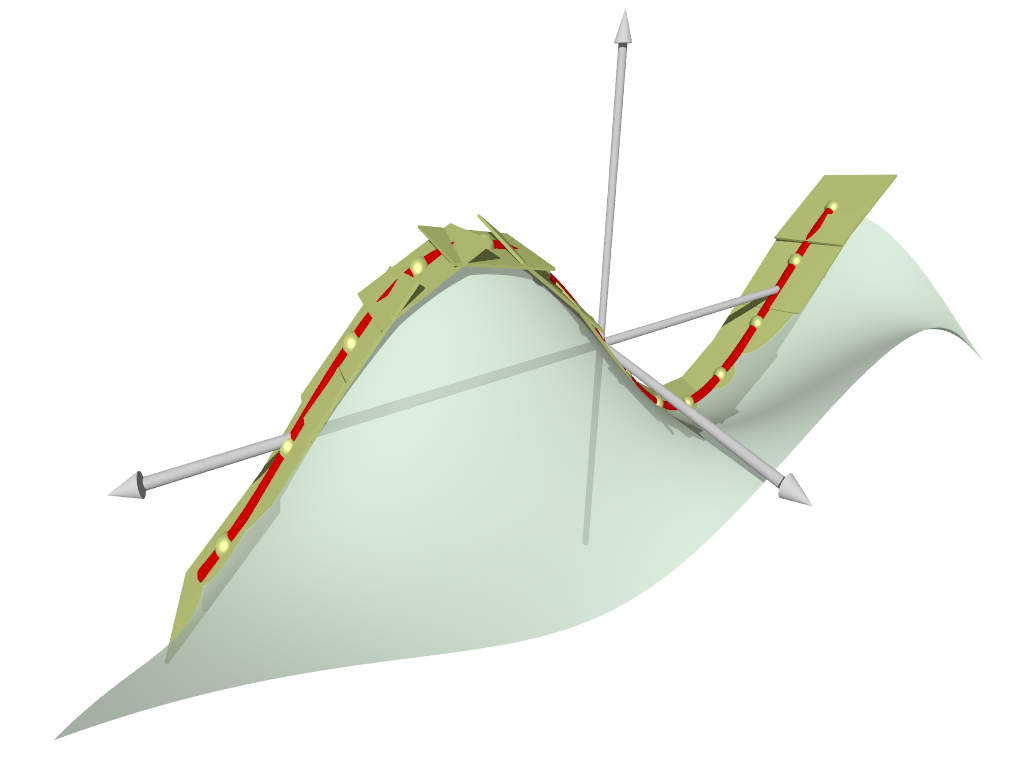
\includegraphics[width=\hsize]{../common/3d/streifen0.png}
\caption{A strip consists of the values and tangent planes
along a curve (red).
The green surface is a solution of the wave equation with the
data of the strip as initial data.
\label{skript:streifen}}
\end{figure}

\begin{figure}
\centering
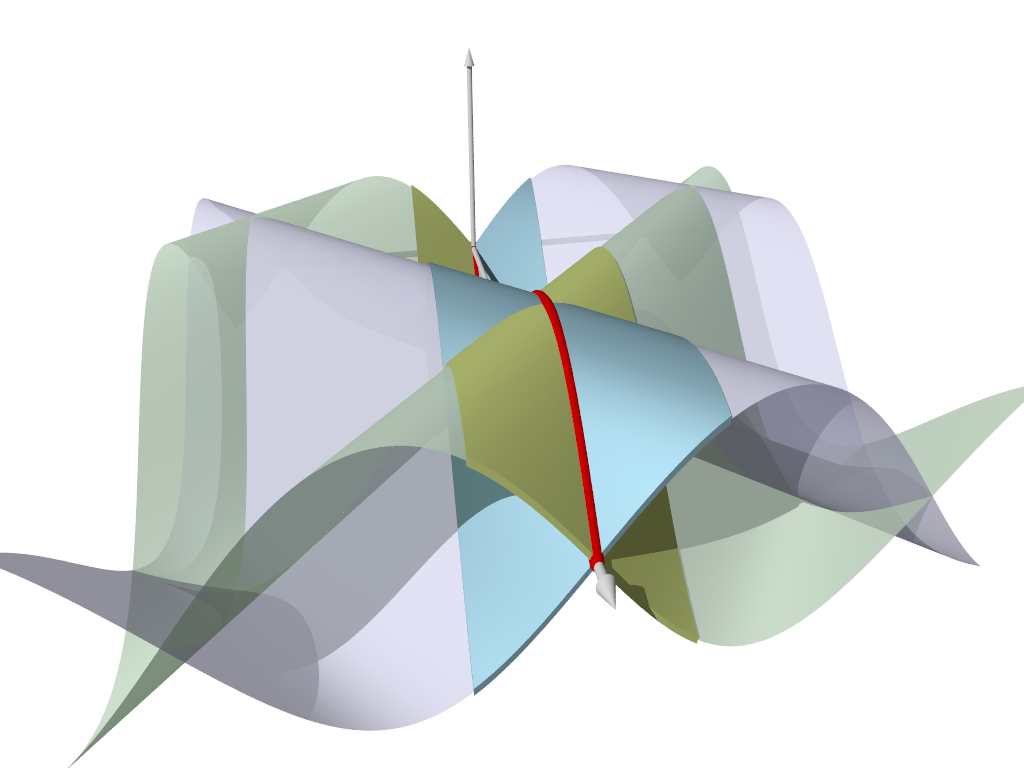
\includegraphics[width=\hsize]{../common/3d/streifen2.png}
\caption{Along the common red curve both solution surfaces have
the same initial values, but different tangent planes, so they
have different strips.
\label{skript:streifen:eindeutig}}
\end{figure}

\begin{figure}
\centering
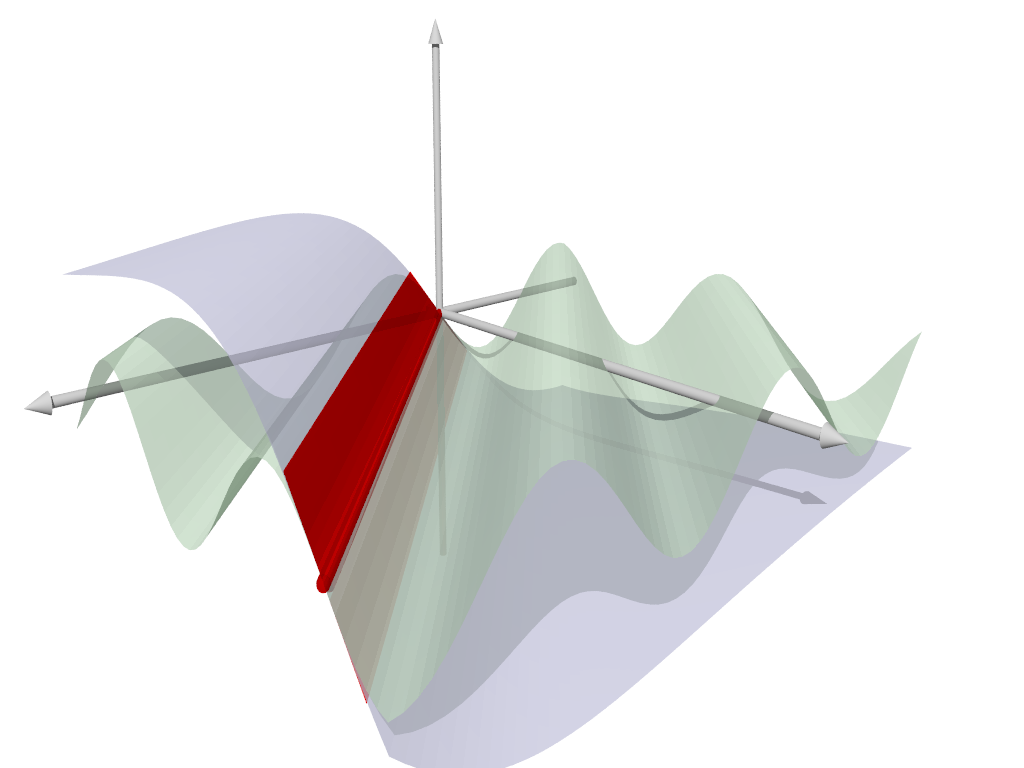
\includegraphics[width=\hsize]{../common/3d/streifen1.png}
\caption{Characteristics are those curves that cannot be used to
define a strip that would uniquely determine the solution surface.
The graph shows two solution of the wave equation with the same
strip: they go through the same curve and they have the same
tangent planes, but the differ in the curvature perpendicular to the
initial curve.
This means that the second order derivatives are not determined by
the equation and the strip data.
\label{skript:streifen:zweideutig}}
\end{figure}

The functions $u(t)$, $p(t)$ and $q(t)$ are not completely arbitrary.
By deriving the first equation \eqref{charanfangs} with respect to $t$,
we find
\[
\dot{u}(t)=\frac{d}{dt}u(t)
=
\frac{d}{dt}u(x(t),y(t))
=
\frac{\partial u}{\partial x}(x(t), y(t))\frac{d}{dt}x(t)
+
\frac{\partial u}{\partial y}(x(t), y(t))\frac{d}{dt}y(t).
\]
Since the partial derivatives are also given in \eqref{charanfangs},
we must also have the relation
\begin{equation}
\dot{u}(t)= p(t)\dot{x}(t) + q(t)\dot{y}(t).
\label{cauchydatarestriction}
\end{equation}

\subsection{Characteristic curves\label{subsection:characteristics-curves}}
Specifying the data of a strip often determines the hyperbolic
partial differential equation uniquely.
In figure~\ref{skript:streifen:eindeutig} two different solutions
are shown that have the same initial curve but different tangent
planes, so the have different strips along this curve.

Deriving the last two equations of \eqref{charanfangs} with respect to $t$,
gives the system of linear equations
\[
\begin{linsys}{3}
\dot p(t)
&=&
\partial_x\partial_xu(x(t),y(t))\,\dot x(t)
&+&
\partial_x\partial_yu(x(t),y(t))\,\dot y(t)
& &
\\
\dot q(t)
&=&
& &
\partial_x\partial_yu(x(t),y(t))\,\dot x(t)
&+&
\partial_y\partial_yu(x(t),y(t))\,\dot y(t)
\end{linsys}
\]
Together with the differential equation we have now three linear equations
to determine the second partial derivatives (colored red)
\[
\begin{linsys}{4}
a{\color{red}\displaystyle\frac{\partial^2 u}{\partial x^2}}
&+&
2b{\color{red}\displaystyle\frac{\partial^2 u}{\partial x\partial y}}
&+&
c{\color{red}\displaystyle\frac{\partial^2 u}{\partial y^2}}
&=&
h(t)\phantom{.}
&=&
g-dp(t)-eq(t)-fu\\
\dot x(t)
{\color{red}\displaystyle\frac{\partial^2 u}{\partial x^2}}
&+&
\dot y(t)
{\color{red}\displaystyle\frac{\partial^2 u}{\partial x\partial y}}
& &
&=&
\dot p(t)\phantom{.}
& &
\\
& &
\dot x(t)
{\color{red}\displaystyle\frac{\partial^2 u}{\partial x\partial y}}
&+&
\dot y(t)
{\color{red}\displaystyle\frac{\partial^2 u}{\partial y^2}}
&=&
\dot q(t).
& &
\end{linsys}
\]
This linear system of equations for the second order derivatives
has the coefficient matrix
\[
\begin{pmatrix}
a&2b&c\\
\dot x(t)&\dot y(t)&0\\
0&\dot x(t)&\dot y(t)
\end{pmatrix}.
\]
The system of equation is not or not uniquely solvable if the
determinant vanishes, i.~e.
\begin{align*}
0&=\left|\begin{matrix}
a&2b&c\\
\dot x(t)&\dot y(t)&0\\
0&\dot x(t)&\dot y(t)
\end{matrix}\right|
\\
&=a\dot y(t)^2-2b\dot x(t)\dot y(t)+c\dot x(t)^2
\end{align*}

\begin{definition}
The characteristics of a differential equation of the form
\eqref{charequation}
are the curves
$t\mapsto(x(t),y(t))$, for which the initial data 
\eqref{charanfangs} does not determine the second partial
derivatives uniquely.
\end{definition}

\begin{satz}
\label{charakteristikendgl}
The characteristics of a partial differential equation
\eqref{charequation}
solve the differential equation
\[
a\dot y(t)^2-2b\dot x(t)\dot y(t)+c\dot x(t)^2=0.
\]
\end{satz}

\subsection{Characteristic strip}
We shoose a characteristic $t\mapsto(x(t),y(t))$.
We are only interested in the case where there are infinitely
many possible values for the second derivative.
This case happens when the determinants
\[
\left|
\begin{matrix}
h&2b&c\\
\dot p(t)&\dot y(t)&0\\
\dot q(t)&\dot x(t)&\dot y(t)
\end{matrix}
\right|
,
\quad
\left|
\begin{matrix}
a&h&c\\
\dot x(t)&\dot p(t)&0\\
0&\dot q(t)&\dot y(t)
\end{matrix}
\right|
,
\quad
\left|
\begin{matrix}
a&2b&h\\
\dot x(t)&\dot y(t)&\dot p(t)\\
0&\dot x(t)&\dot q(t)
\end{matrix}
\right|
\]
all vanish, where $h=g-dp(t)-eq(t)-fu(x(t),y(t))$.
It suffices the select a single one of those determinants,
we choose the second:
\begin{align*}
a\dot p(t)\dot y(t)-h\dot x(t)\dot y(t)+c\dot x(t)\dot q(t)&=0
\end{align*}

Together with the condition~\eqref{cauchydatarestriction}
we now have three equations that the functions
$x$, $y$, $u$, $p$ and $q$ must satisfy in order for the second
derivatives to not be determined uniquely by the initial data.

\begin{definition}
A strip along a characteristic which satisfies
\[
a\dot p(t)\dot y(t)-h\dot x(t)\dot y(t)+c\dot x(t)\dot q(t)=0
\]
is called a {\em characteristic strip}.
\end{definition}

Thus it is also possible that the integral surfaces of a partial
differential equation touch along a curve, but are different
nevertheless.
By necessity, the tangent planes along the intersection curve form
a characteristic strip.

\begin{satz}
\label{skript:satz:charakteristiken}
If two different integral surfaces touch along a curve,
then this curve together with the tangent planes form a characteristic strip.
\end{satz}

Figure~\ref{skript:streifen:zweideutig} shows two solutions of the wave
equation that touch along a characteristic.
From theorem~\ref{skript:satz:charakteristiken} the red strip is a 
characteristic strip.

\begin{proof}
Apparently there are at least two different solutions of the
partial differential equation that contain the curve which in
addition have the same tangent planes.
The curve and the tangent planes do not determine the solution
uniquely, so they form a characteristic strip.
\end{proof}

\subsection{Examples}
\subsubsection{Wave equation}
The characteristics of the wave equation
\begin{equation}
\partial_t^2u-a^2\partial_x^2u=0
\label{hyperbolisch:wellengleichung}
\end{equation}
are the curves $s\mapsto(t(s),x(s))$, that satisify the equation
\begin{align*}
\left(
\frac{dx(s)}{ds}\right)^2-a^2\left(\frac{dt(s)}{ds}\right)^2&=0
\\
\frac{dx(s)}{ds}
&=
\pm a\frac{dt(s)}{ds}
\\
\Rightarrow
\frac{dx}{dt}=\pm a.
\end{align*}
These are straight lines with slope $\pm a$.
\begin{figure}
\centering
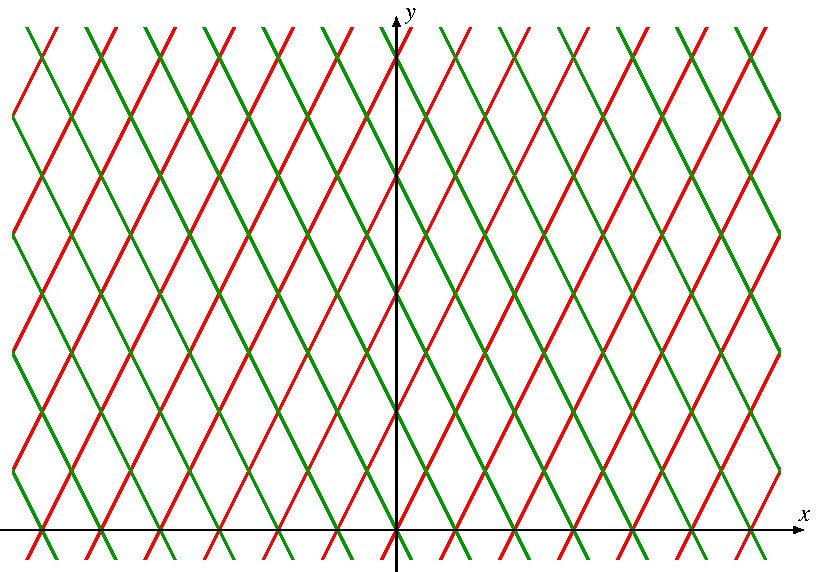
\includegraphics{9-hyperbolic/images/wavechar.pdf}
\caption{Characteristics of the wave
equation~(\ref{hyperbolisch:wellengleichung})
\label{hyp:wellen}}
\end{figure}
Figure~\ref{hyp:wellen} shows the characteristics.

\subsubsection{The equation $\partial_x\partial_yu=0$}
The condition for the characteristics in this case is
\[
-\dot x(t)\dot y(t)=0
\]
One of the derivatives must disappear, which is only possible for
curves that are parallel to the $x$- or the $y$-axis.
Figure~\ref{hyp:dxdy} shows these characteristics
\begin{figure}
\centering
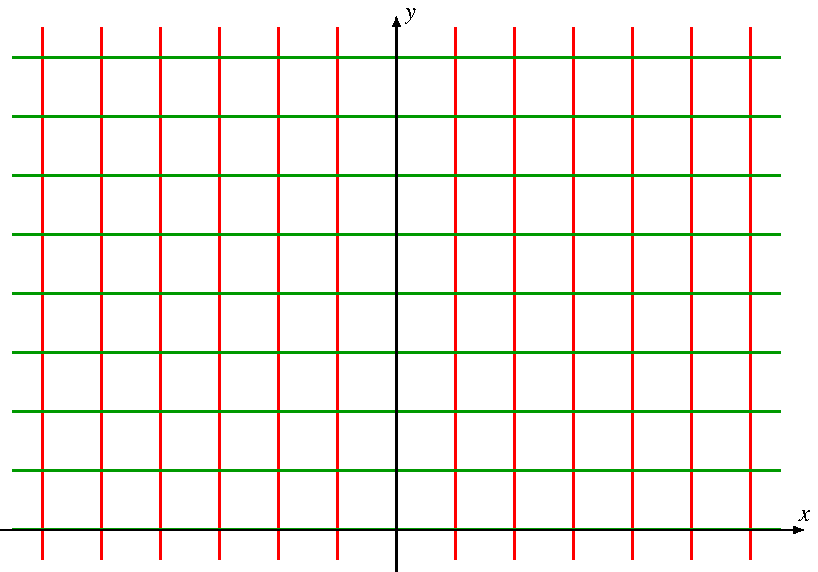
\includegraphics{9-hyperbolic/images/dxdy.pdf}
\caption{characteristics of the hyperbolic partial differential equation
$\partial_x\partial_yu=0$.
\label{hyp:dxdy}}
\end{figure}

\subsubsection{Curved characteristics}
The partial differential equation
\begin{equation}
\partial_t^2u-x^2\partial_x^2u=0
\label{hyperbolisch:gekruemmt}
\end{equation}
is hyperbolic for $x\ne 0$.
The characteristics satisfy the equation
\begin{align*}
x'(s)^2-x^2t'(s)^2&=0
\\
xt'&=\pm  x'
\\
\frac{d}{ds}t&=\pm\frac{d}{ds}\log x
\\
t&=\pm\log x+C
\\
x&=x_0e^{\pm t}
\end{align*}
The characteristics are exponential curves.
In figure \ref{hyp:exp}
the characteristics for the positive sign are drawn in red,
the characteristics for the negative sign green.
\begin{figure}
\centering
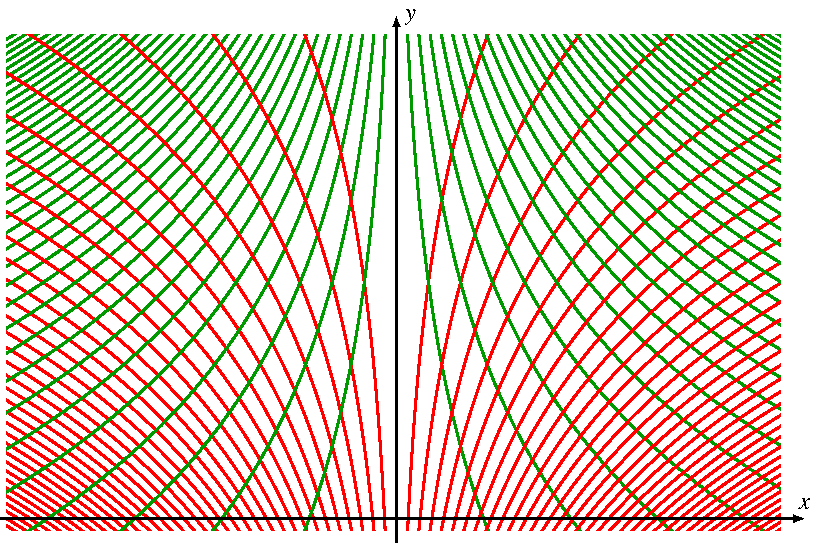
\includegraphics{9-hyperbolic/images/exponential.pdf}
\caption{Characteristics for $x\ne 0$ for the hyperbolic partial
differential equation~\eqref{hyperbolisch:gekruemmt}.
\label{hyp:exp}}
\end{figure}

This equation describes a wave equation in a medium in which
the wave velocity increases with increasing $x$.
The exponential curves suggest that the wave becomes faster when moving ``out''.

\subsection{Characteristics of elliptic or parabolic partial differential
equations}
The theory of the characteristics developed above can also be
applied to elliptic or hyperbolic partial differential equations.

In the elliptic case, the differential equation of the characteristics
\[
a\dot y(t)^2-2b\dot x(t)\dot y(t)+c\dot x(t)^2=0
\]
does not have any solutions, as the expression only vanishes only for
$\dot x(t)=0$ and $\dot y(t)=0$.

For parabolic partial differential equations the characteristic
equation becomes in a suitable coordinate system
\[
-\kappa t'(s)^2=0.
\]
This can only hold true if $t$ is constant.
The characteristics in this case are straight lines parallel
to the $x$-axis.
In fact it is not possible to determine the second derivative
with respect to $t$ for initial data along a line parallel
to the $x$-axis.

We will summarize the information about causality or which points on
the boundery can influence the solution in which points of the domain
in section~\ref{section:which-boundary-points}

\subsection{Some interesting theorems}

\begin{satz}
Every integral surface can be covered with a set of characteristic
strips.
\end{satz}

\begin{proof}
Let $u$ be the solution of a partial differential equation.
The differential equation in theorem~\ref{charakteristikendgl}
describes two curves $t\mapsto(x(t),y(t))$ in every point of the domain.
Obviously it is possible to cover the solution surface by such curves.
By substituting these curves into $u(x,y)$, $\partial_xu(x,y)$
and $\partial_yu(x,y)$ we get a set of characteristic strips
as claimed.
\end{proof}

\begin{satz}
If a set of characteristic strips covers a surface $S$ defined
by the function $u(x,y)$ and this function has continuous 
second derivatives then $u$ is a solution of the differential equation.
\end{satz}

\begin{proof}
The characteristic strips satisfy the equations
\begin{equation}
\begin{gathered}
a\dot y(t)^2-2b\dot x(t)\dot y(t)+c\dot x(t)^2=0,
\\
a\dot p(t)\dot y(t)-h\dot x(t)\dot y(t)+c\dot x(t)\dot q(t)=0,
\\
\dot u(t)=p(t)\dot x(t)+q(t)\dot y(t).
\end{gathered}
\label{alle}
\end{equation}
Let's call the second derivatives of $u$ along a cahracteristic curve
\begin{align*}
R&=\partial_x^2u(x(t),y(t)),
\\
S&=\partial_x\partial_yu(x(t),y(t)),
\\
T&=\partial_y^2u(x(t),y(t)).
\end{align*}
We can write
\begin{align*}
\dot p(t)&=R(t)\dot x(t)+S(t)\dot y(t)\qquad\text{and}\\
\dot q(t)&=S(t)\dot x(t)+T(t)\dot y(t).
\end{align*}
If we substitute this in the second equation of \eqref{alle}, we get
\begin{align*}
a(R\dot x+S\dot y)\dot y-h\dot x\dot y+c\dot x(S\dot x+T\dot y)&=0
\\
\Rightarrow \qquad(aR-h+cT)\dot x\dot y+aS\dot y^2 +cS \dot x^2&=0.
\end{align*}
Multiplying the first equation of
\eqref{alle} by $t$ and subtracting it we get
\[
(aR+2bS+cT-h)\dot x\dot y=0.
\]
Writing out the parenthesis leads to the equation
\[
a\partial_x^2u+2b\partial_x\partial_yu+c\partial_y^2u-h=0
\]
which is the original differential equation.
\end{proof}
This theorem teaches that the hyperbolic partial differential equation
can be solved by looking for characteristic strips.
for this it suffices the solve ordinary differential equations for the
functions $x$, $y$, $p$, $q$, $R$, $S$ and $T$.



%
% linearization.tex -- XXX
%
% (c) 2019 Prof Dr Andreas Mueller, Hochschule Rapperswil 
%
\section{Linearisierung}
\rhead{Linearisierung}
In einigen Fällen sind Lösungen einer nichtlinearen PDGL gesucht, die 
nur wenig von einer bekannten Lösung abweichen. Beispielsweise ändert
ein stromlinienförmig gebautes Flugzeug bei hoher Geschwindigkeit die
Strömung nur vergleichsweise wenig. Man kann daher versuchen, aus der
nichtlinearen Gleichung eine lineare Gleichung für die Abweichung
von der bekannten Lösung abzuleiten. Dieses Verfahren wird oft auch
Störungstheorie genannt.

\subsection{Das allgemeine Vorgehen}
Der Einfachheit halber führen wir das Verfahren nur für Gleichungen
erster Ordnung in zwei Variablen durch. Eine solche PDGL kann mit Hilfe
einer Funktion $F(x,y,u,p,q)$ von fünf Variablen geschrieben werden als
\begin{equation}
F(x,y,u(x,y), \partial_xu(x,y),\partial_yu(x,y))=0.
\label{nichtlinear}
\end{equation}
Sei $u(x,y)$ eine Lösung der Gleichung (\ref{nichtlinear}). Wir suchen
jetzt weitere Lösungen der Gleichung, die sich jedoch nur wenig von
$u$ unterscheiden dürfen. Wir setzen diese Lösungen in der Form
\begin{equation}
u(x,y)+av(x,y)
\label{linearisierungansatz}
\end{equation}
an, wobei der Parameter $a$ dazu dienen soll, die den
zweiten Term beliebig klein machen zu können. Wir möchten eine Gleichung
für $v(x,y)$ aufstellen.

Wir setzen den Ansatz (\ref{linearisierungansatz}) in die Gleichung
ein, und erhalten
\[
F(x,y,u(x,y)+av(x,y),\partial_xu(x,y)+a\partial_xv(x,y),
\partial_yu(x,y)+a\partial_yv(x,y))=0
\]
Für $a=0$ ist die Gleichung erfüllt, wir suchen ein $v$ so dass die Gleichung
für kleine $a$ näherungsweise auch erfüllt ist. Dies erreichen wir,
indem wir nach $a$ ableiten:
\begin{align*}
0&=
\left.\frac{d}{da}
F(x,y,u(x,y)+av(x,y),\partial_xu(x,y)+a\partial_xv(x,y),
\partial_yu(x,y)+a\partial_yv(x,y))\right|_{a=0}
\\
&=F(x,y,u(x,y),\partial_xu(x,y),\partial_yu(x,y))
\\
&\qquad
+
\partial_uF(x,y,u(x,y),\partial_xu(x,y),\partial_yu(x,y))\cdot v(x,y)
\\
&\qquad
+
\partial_pF(x,y,u(x,y),\partial_xu(x,y),\partial_yu(x,y))\cdot \partial_xv(x,y)
\\
&\qquad
+
\partial_qF(x,y,u(x,y),\partial_xu(x,y),\partial_yu(x,y))\cdot \partial_yv(x,y)
\end{align*}
Der erste Term fällt weg, weil $u$ bereits eine Lösung ist,
es bleibt eine lineare PDGL für $v$:
\begin{align*}
0&=
\partial_uF(x,y,u(x,y),\partial_xu(x,y),\partial_yu(x,y))\cdot v(x,y)
\\
&\qquad
+
\partial_pF(x,y,u(x,y),\partial_xu(x,y),\partial_yu(x,y))\cdot \partial_xv(x,y)
\\
&\qquad
+
\partial_qF(x,y,u(x,y),\partial_xu(x,y),\partial_yu(x,y))\cdot \partial_yv(x,y)
\end{align*}
Etwas allgemeiner könnte auch noch die Funktion $F$ von $a$ abhängen,
also $F(a,x,y,u,p,q)$. In diesem Fall wird die Ableitung nach $a$ an
der Stelle $a=0$ zu
\begin{align*}
0&=
\left.\frac{d}{da}
F(x,y,u(x,y)+av(x,y),\partial_xu(x,y)+a\partial_xv(x,y),
\partial_yu(x,y)+a\partial_yv(x,y))\right|_{a=0}
\\
&=
F(0,x,y,u(x,y),\partial_xu(x,y),\partial_yu(x,y))
\\
&\qquad
+\partial_aF(0,x,y,u(x,y),\partial_xu(x,y),\partial_yu(x,y))
\\
&\qquad
+
\partial_uF(a,x,y,u(x,y),\partial_xu(x,y),\partial_yu(x,y))\cdot v(x,y)
\\
&\qquad
+
\partial_pF(a,x,y,u(x,y),\partial_xu(x,y),\partial_yu(x,y))\cdot \partial_xv(x,y)
\\
&\qquad
+
\partial_qF(a,x,y,u(x,y),\partial_xu(x,y),\partial_yu(x,y))\cdot \partial_yv(x,y)
\end{align*}
Die lineare PDGL ist in diesem Fall
\begin{align*}
0
&=
\partial_aF(0,x,y,u(x,y),\partial_xu(x,y),\partial_yu(x,y))
\\
&\qquad
+
\partial_uF(x,y,u(x,y),\partial_xu(x,y),\partial_yu(x,y))\cdot v(x,y)
\\
&\qquad
+
\partial_pF(x,y,u(x,y),\partial_xu(x,y),\partial_yu(x,y))\cdot \partial_xv(x,y)
\\
&\qquad
+
\partial_qF(x,y,u(x,y),\partial_xu(x,y),\partial_yu(x,y))\cdot \partial_yv(x,y)
\end{align*}
Jede Lösung der nichtlinearen Gleichung gibt also Anlass zu Lösungen
in ``unmittelbarer'' Nähe, welche aus der linearisierten Gleichung
gefunden werden können.

\subsection{Linearisierung von PDGL zweiter Ordnung}
Eine PDGL zweiter Ordnung ist gegeben durch eine Funktion von neun
Variablen
\[
F(x,y,u,p,q,r,s,t),
\]
in die man die Funktionswerte und die Ableitungen einsetzt:
\[
F(x,y,u(x,y), \partial_xu(x,y),\partial_yu(x,y),
\partial_x^2u(x,y),
\partial_x\partial_yu(x,y),
\partial_y^2u(x,y))
=0
\]
Um die linearisierte PDGL zu finden, geht man wieder von einer
Lösung $u(x,y)$ aus, und sucht eine ``Nachbarlösung'' in der
Form $u(x,y)+av(x,y)$. Diesen Ansatz setzt man in die 
Differentialgleichung ein und leitet an der Stelle $a=0$
nach $a$ ab. Wie im Falle der Gleichung erster Ordnung kann auch
hier der Parameter $a$ auch in $F$ vorkommen, wir führen gleich
von Anfang an diesen allgemeineren Fall  durch:
\begin{align*}
0&=
\frac{d}{da}
F(a,x,y,u(x,y), \partial_xu(x,y)+a\partial_xv(x,y),\partial_yu(x,y)+a\partial_yv(x,y),
\\
&\qquad
\partial_x^2u(x,y)+a\partial_x^2v(x,y),
\partial_x\partial_yu(x,y)+a\partial_x\partial_yv(x,y),
\partial_y^2u(x,y)+a\partial_y^2v(x,y))\bigg|_{a=0}
\\
&=
F(x,y,u(x,y), \partial_xu(x,y),\partial_yu(x,y),
\partial_x^2u(x,y),
\partial_x\partial_yu(x,y),
\partial_y^2u(x,y))
\\
&\qquad+
\partial_a
F(0,x,y,u(x,y), \partial_xu(x,y),\partial_yu(x,y),
\partial_x^2u(x,y),
\partial_x\partial_yu(x,y),
\partial_y^2u(x,y))
\\
&\qquad+
\partial_u
F(0,x,y,u(x,y), \partial_xu(x,y),\partial_yu(x,y),
\partial_x^2u(x,y),
\partial_x\partial_yu(x,y),
\partial_y^2u(x,y))\cdot v(x,y)
\\
&\qquad+
\partial_p
F(0,x,y,u(x,y), \partial_xu(x,y),\partial_yu(x,y),
\partial_x^2u(x,y),
\partial_x\partial_yu(x,y),
\partial_y^2u(x,y))\cdot \partial_xv(x,y)
\\
&\qquad+
\partial_q
F(0,x,y,u(x,y), \partial_xu(x,y),\partial_yu(x,y),
\partial_x^2u(x,y),
\partial_x\partial_yu(x,y),
\partial_y^2u(x,y))\cdot \partial_yv(x,y)
\\
&\qquad+
\partial_q
F(0,x,y,u(x,y), \partial_xu(x,y),\partial_yu(x,y),
\partial_x^2u(x,y),
\partial_x\partial_yu(x,y),
\partial_y^2u(x,y))\cdot \partial_x^2v(x,y)
\\
&\qquad+
\partial_r
F(0,x,y,u(x,y), \partial_xu(x,y),\partial_yu(x,y),
\partial_x^2u(x,y),
\partial_x\partial_yu(x,y),
\partial_y^2u(x,y))\cdot \partial_x\partial_yv(x,y)
\\
&\qquad+
\partial_s
F(0,x,y,u(x,y), \partial_xu(x,y),\partial_yu(x,y),
\partial_x^2u(x,y),
\partial_x\partial_yu(x,y),
\partial_y^2u(x,y))\cdot \partial_y^2v(x,y)
\end{align*}

\subsection{Linearisierung der Burgers Gleichung}
Wir wenden das Linearisierungsverfahren auf die Gleichung von Burgers an.
Wir schreiben sie zur leichteren Übertragbarkeit der Formeln
mit $x$ und $y$ als unabhängige Variablen anstellen von $x$ und $t$,
wir suche also Lösungen der Differentialgleichung
\[
\partial_yu-u\partial_xu-\partial_x^2u=0
\]
Die Funktion $F$ ist in diesem Fall
\[
F(x,y,u,p,q,r,s,t)=q-r-up.
\]
Die Linearisierungsformeln sagen, dass wir die Ableitungen von $F$ nach
den Variablen verwenden müssen als Koeffizienten der Ableitungen,
für die die Variablen stehen.  Dabei müssen wir in die partiellen Ableitungen
von $F$ jeweils die Lösung $u$ bzw.~ihre partiellen Ableitungen einsetzen.
Die Koeffizienten sind
\begin{align*}
\partial_uF&=-p=-\partial_xu(x,y)
\\
\partial_pF
&=-u=-u(x,y)
\\
\partial_qF
&=1
\\
\partial_rF
&=-1
\end{align*}
alle anderen partiellen Ableitungen von $F$ verschwinden. Die linearisierte
Gleichung lautet also
\begin{align*}
-\partial_xu(x,y)\cdot v(x,y)
-
u(x,y)\cdot\partial_xv(x,y)
+\partial_yv(x,y)
-\partial_x^2v(x,y)=0,
\end{align*}
eine parabolische PDGL. In den ursprünglichen Koordinaten und der
üblichen Reihenfolge der Ableitungen geschrieben
lautet sie
\[
-\partial_x^2v(t,x)
+\partial_tv(t,x)
+ u(t,x)\cdot\partial_xv(t,x)
+\partial_xu(t,x)\cdot v(t,x)
=0,
\]

\subsubsection{Konstante Geschwindigkeit}
Die konstante Funktion $u(t,x)=c$ ist eine Lösung der nichtlinearen
Gleichung. Die linearisierte Gleichung wird damit zu
\[
\partial_tv
-\partial_x^2v
-c\partial_xv=0.
\]
Leider ist diese Gleichung auch noch nicht direkt in einer Form,
in der wir sie lösen können. Schreiben wir die gesuchte Funktion
in der Form
\[
v(t,x)=w(t,x+ct)
\]
und bezeichnen die partiellen Ableitungen von $w$ nach der ersten
und zweiten Variablen mit $\partial_1w$ bzw.~$\partial_2w$, dann
erhalten wir zunächst die partiellen Ableitungen von $v$
in der Form
\begin{align*}
\partial_t v(t,x)&=\partial_1w(t,x+ct)+c\partial_2w(t,x+ct)
\\
\partial_x v(t,x)&=\partial_2w(t,x+ct)
\\
\partial_x^2v(t,x)&=\partial_2^2w(t,x+ct)
\end{align*}
In die PDGL eingesetzt erhalten wir
\begin{align*}
0&=
\partial_t v(t,x)
-\partial_x^2v(t,x)
-c\partial_x v(t,x)
\\
&=
\partial_1w(t,x+ct)+c\partial_2w(t,x+ct)
-\partial_2^2w(t,x+ct)
-c\partial_2w(t,x+ct)
\\
&=\partial_1w(t,x+ct)-\partial_2w(t,x+ct)
\end{align*}
Die Funktion $w$ ist also eine Lösung der Wärmeleitungsgleichung.

\subsubsection{Lösungen der linearisierten Gleichung}
Die Wärmeleitungsgleichung hat die Standardlösungen
\[
w(t,x)=\frac1{\sqrt{t}}e^{-\frac{(x-\xi)^2}{4t}},
\]
die man durch Nachrechnen unmittelbar bestätigen kann:
\begin{align*}
\partial_t w(t,x)
&=
\left(
-\frac1{2t^{\frac32}}
+\frac{(x-\xi)^2}{4t^{\frac52}}
\right)e^{-\frac{x^2}{4t}}
\\
\partial_x w(t,x)
&=
-\frac{(x-\xi)}{2t^{\frac32}}
e^{-\frac{x^2}{4t}}
\\
\partial_x^2w(t,x)
&=
\left(
\frac{(x-\xi)^2}{4t^{\frac52}}
-\frac{1}{2t^{\frac32}}
\right)e^{-\frac{x^2}{4t}}
\\
\partial_tw(t,x)-\partial_x^2w(t,x)
&=
\left(
-\frac1{2t^{\frac32}}
+\frac{(x-\xi)^2}{4t^{\frac52}}
-\frac{(x-\xi)^2}{4t^{\frac52}}
+\frac{1}{2t^{\frac32}}
\right)e^{-\frac{(x-\xi)^2}{4t}}=0
\end{align*}
Als Lösungen der linearisierten Gleichung kommen also Funktionen der
Form
\[
v(t,x)=\frac1{\sqrt{t}}e^{-\frac{(x-\xi+ct)^2}{4t}}
\]
oder Überlagerungen derselben in Frage.

\subsubsection{Stabilität der Strömung}
Die im vorangegangenen Abschnitt abgeleiteten Lösung der linearisierten
Gleichung lässt sich auch so interpretieren: eine kleine Störung zur Zeit
$t=0$ wird Anlass zu einem mit Geschwindigkeit $c$ nach links
laufenden gaussschen Wellenbuckel Anlass geben. Dieser Buckel wird mit
der Zeit immer flacher und ausgedehnter werden. Insbesondere verschwinden
kleine Störungen mit der Zeit wieder, die Strömung ist also stabil.

Tritt jedoch eine Störung auf, die so gross ist, dass die Linearisierung
nicht mehr anwendbar ist, dann werden neue Phänomene auftreten, insbesondere kann
die Strömung instabil sein. Störungen können sich aufschaukeln bis die
Lösung nicht mehr stetig ist (Geschwindigkeitssprünge, Schockwellen)
oder die Geschwindigkeit könnte unvorhersagbar zu schwanken beginnen
(Turbulenz).

Alternativ könnte man auch mit dem Maximumprinzip argumentieren: Extremwerte
sind in der Anfangsbedingung zu finden, eine Störung muss also mit der
Zeit immer schwächer werden.

\subsubsection{Ansteigende Geschwindigkeit}
Wir untersuchen diese Gleichung noch für den Fall der bereits 
früher untersuchten speziellen Lösung 
\[
u(t,x)=\frac{A-x}{B+t}
\]
explizit aufschreiben. Dazu benötigen wir die partielle Ableitung
nach $x$, die wir ebenfalls bereits früher berechnet haben:
\begin{align*}
\partial_x u(t,x)&=-\frac{1}{B+t}
\end{align*}
Die linearisierte Gleichung wird damit zu
\begin{align*}
-\partial_x^2v(t,x)
+\partial_tv(t,x)
+ \frac{A-x}{B+t}\partial_xv(t,x)
-\frac{1}{B+t} v(t,x)
&=0
\\
-(B+t)\partial_x^2v(t,x)
+(B+t)\partial_tv(t,x)
+ (A-x)\partial_xv(t,x)
- v(t,x)
&=0
\end{align*}
Leider lässt sich in diesem Fall nicht so offensichtlich eine Lösung finden.


%
% singularities.tex -- XXX
%
% (c) 2019 Prof Dr Andreas Mueller, Hochschule Rapperswil 
%
\section{Entstehung von Singularitäten\label{burgersunstetig}}
\rhead{Singularitäten}
\begin{figure}
\begin{center}
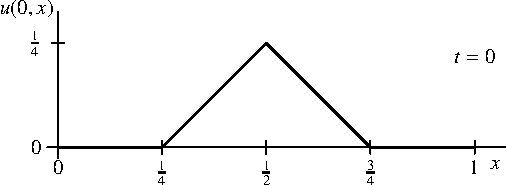
\includegraphics[width=0.8\hsize]{../common/images/burgers-1}
\end{center}
\caption{Anfangsbedingung für die Burgers Gleichung einer idealen
Flüssigkeit\label{burgersanfang}}
\end{figure}
In diesem Abschnitt möchten wir die Burgers Gleichung für die ideale
Flüssigkeit
\[
\frac{\partial}{\partial t}u+\frac{\partial}{\partial x}\left(\frac{u^2}2\right)=0
\]
auf dem Interval $x\in[0,1]$ und für $t>0$
mit der Anfangsbedingung
\[
u(0,x)=\begin{cases}
0\qquad&\text{$x<\frac14$ oder $x>\frac34$}\\
x-\frac14\qquad&\frac14\le x\le \frac12\\
\frac34-x\qquad&\frac12\le x\le \frac34
\end{cases}
\]
lösen (siehe Abbildung \ref{burgersanfang}).

\begin{figure}
\begin{center}
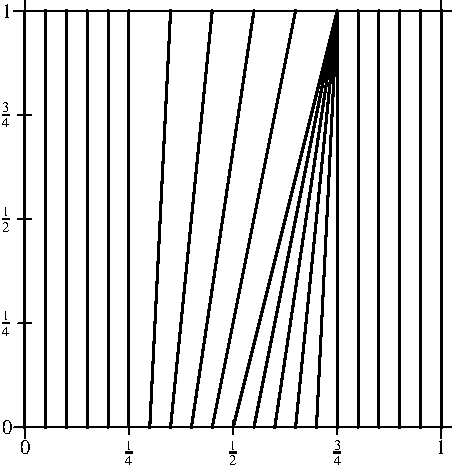
\includegraphics[width=0.8\hsize]{../common/images/burgers-2}
\end{center}
\caption{Niveaulinien (Charakteristiken) der Lösung der Burgers-Gleichung für
die ideale Flüssigkeit\label{burgersniveau}}
\end{figure}
Die Differentialgleichung ist von erster Ordnung, in der Form
\[
\partial_tu+u\partial_xu=0
\]
haben wir die zugehörige geometrische Theorie in Abschnitt
\ref{pdgl1ordnung} besprochen. Dort wurde darauf hingewiesen,
dass der Vektor 
\[
\begin{pmatrix}
1\\u\\0
\end{pmatrix}
\]
immer an die Fläche $u=u(t,x)$ tangential ist. Die Lösungsfläche
entsteht dadurch, dass die Anfangsbedingung mit Hilfe dieses Vektors
verschoben wird. 
Der Punkt $(0,x,u(0,x))$ entwickelt sich nach dieser Methode zu
Punkten $(t,x+u(0,x)t, u(0,x))$ der Lösungsfläche. Die Kurven
gleichen Funktionswertes bilden also Geraden, deren Steigung im
$x$-$t$-Koordinatensystem $u(0,t)^{-1}$ ist. Die Niveaulinien der
Lösung sehen daher aus wie in der Abbildung \ref{burgersniveau}
dargestellt.
Daraus kann man jetzt auch die Lösungen ablesen. In der Abbildung
\ref{burgerssprung} kann man die Entwicklung der Spitze zu einem
Sprung an der Stelle $x=\frac34$ beobachten.

\begin{figure}
\begin{center}
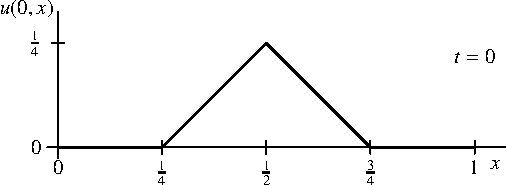
\includegraphics[width=0.8\hsize]{../common/images/burgers-1}
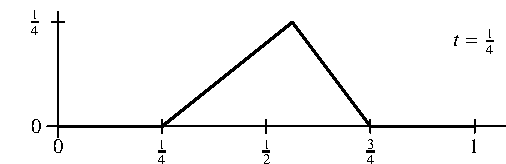
\includegraphics[width=0.8\hsize]{../common/images/burgers-3}
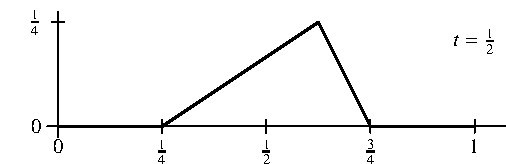
\includegraphics[width=0.8\hsize]{../common/images/burgers-4}
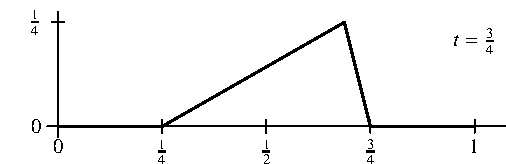
\includegraphics[width=0.8\hsize]{../common/images/burgers-5}
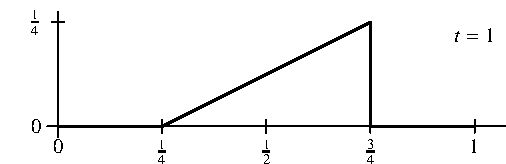
\includegraphics[width=0.8\hsize]{../common/images/burgers-6}
\end{center}
\caption{Entwicklung eines Sprungs in der Lösung der Gleichung von Burgers\label{burgerssprung}}
\end{figure}

Man könnte argumentieren, dass die Anfangsbedingung ja bereits nicht differenzierbar
ist, und dass die Lösungen dies ebenfalls nicht sind. Man kann
jedoch eine beliebige glatte Funktion als Anfangsbedingung wählen, welche
innerhalb des Intervals $[\frac14,\frac12]$ monoton von $0$ auf $\frac14$ 
ansteigt, im Punkt $x=\frac12$ den maximalen Wert $\frac14$ annimmt,
und im Interval $[\frac12,\frac34]$ monoton auf $0$ abfällt.
Das Maximum wird sich entlang der Charakteristiken zum Punkt
$(1,\frac34,\frac14)$ entwicklen. Der Funktionswert $u(0,x)$ im Punkt $(0,x)$
für $x\in[\frac14,\frac12]$ ist derselbe wie im Punkt $(1,x+u(0,x))$.
Der Funktionsgraph $x\mapsto u(1,x)$ hat also die Parameterdarstellung
\[
[{\textstyle\frac14},{\textstyle\frac12}]\to\mathbb R\colon s\mapsto (s+u(0,s),u(0,s))
\]
Diese ist jedenfalls eine glatte Funktion. Andererseits komprimieren
die Charakteristiken das Interval $[\frac12,\frac34]$ auf
den Punkt $(1,\frac34)$ so dass bei $x=\frac34$ wieder ein Sprung entsteht.



